\documentclass[border=2pt]{standalone}
\usepackage{tikz}
\usetikzlibrary{arrows.meta}
\definecolor{current}{HTML}{0072B2}
\definecolor{voltage}{HTML}{CC79A7}

% TUNABLES: approximately 183 mm wide; block and terminal positions below.
\newcommand{\bodyfont}{\fontsize{9}{11}\selectfont}
\begin{document}
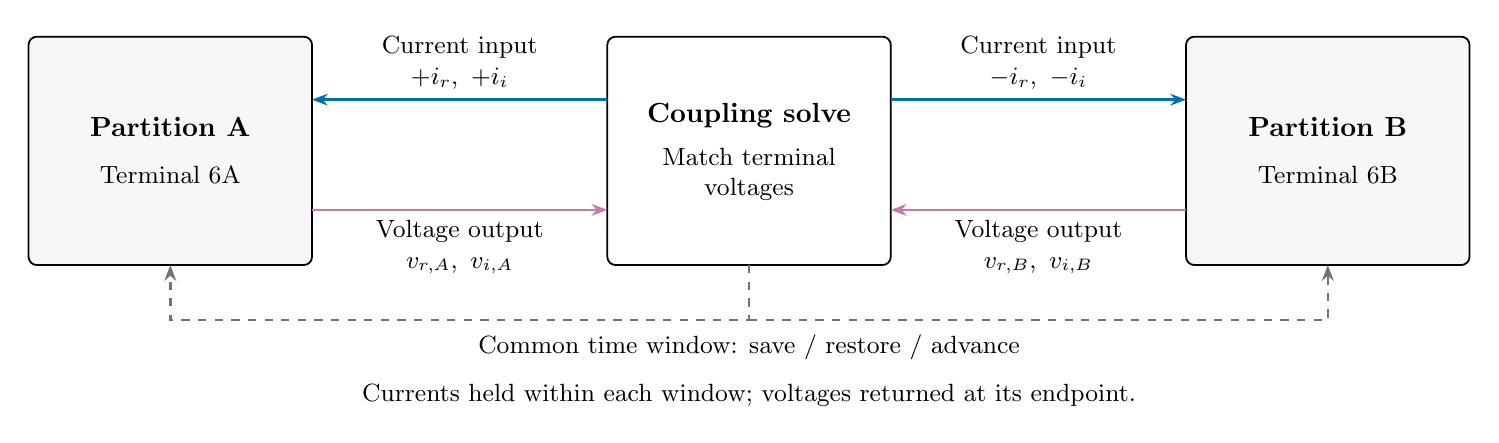
\begin{tikzpicture}[x=1cm,y=1cm,font=\bodyfont,line width=0.65pt,
  signal/.style={-{Stealth[length=2mm]},line width=0.9pt},
  control/.style={signal,dashed,black!55}]
\draw[rounded corners=3pt,fill=black!3] (0,0) rectangle (3.6,2.9);
\draw[rounded corners=3pt] (7.35,0) rectangle (10.95,2.9);
\draw[rounded corners=3pt,fill=black!3] (14.7,0) rectangle (18.3,2.9);

\node[font=\bfseries] at (1.8,1.75) {Partition A};
\node at (1.8,1.15) {Terminal 6A};
\node[font=\bfseries] at (9.15,1.9) {Coupling solve};
\node[align=center] at (9.15,1.15) {Match terminal\\voltages};
\node[font=\bfseries] at (16.5,1.75) {Partition B};
\node at (16.5,1.15) {Terminal 6B};

\draw[signal,current] (7.35,2.1) --
  node[above,align=center,text=black] {Current input\\$+i_r,\ +i_i$} (3.6,2.1);
\draw[signal,current] (10.95,2.1) --
  node[above,align=center,text=black] {Current input\\$-i_r,\ -i_i$} (14.7,2.1);
\draw[signal,voltage] (3.6,0.7) --
  node[below,align=center,text=black] {Voltage output\\$v_{r,A},\ v_{i,A}$} (7.35,0.7);
\draw[signal,voltage] (14.7,0.7) --
  node[below,align=center,text=black] {Voltage output\\$v_{r,B},\ v_{i,B}$} (10.95,0.7);

\draw[control] (9.15,0) -- (9.15,-0.7) -- (1.8,-0.7) -- (1.8,0);
\draw[control] (9.15,-0.7) -- (16.5,-0.7) -- (16.5,0);
\node at (9.15,-1.05) {Common time window: save / restore / advance};
\node at (9.15,-1.65) {Currents held within each window; voltages returned at its endpoint.};
\end{tikzpicture}
\end{document}
